\section{paleoTS}

\subsubsection*{Europe, genera, continental}\label{europe-genera-continental}

\begin{longtable}[]{@{}rrrr@{}}
	\caption[PaleoTS object of continental \T in Europe]{PaleoTS object of continental testudinids in Europe. Mean Age (tt), sample size (nn), mean carapace lengths (mm) and variance (vv) are shown. Largest mean carapace length occurs in the Lower Pliocene and Lower Pleistocene.}
	\label{tab:pTSEuC}\tabularnewline
	\toprule
	tt & nn & mm & vv\tabularnewline
	\midrule
	\endfirsthead
	\toprule
	tt & nn & mm & vv\tabularnewline
	\midrule
	\endhead
	0.00585 & 2 & 149.5381 & 3450.8267\tabularnewline
	0.06885 & 1 & 187.0000 & 0.0000\tabularnewline
	0.45350 & 2 & 205.4750 & 198.0050\tabularnewline
	1.29350 & 2 & 204.9292 & 23.1767\tabularnewline
	2.19700 & 1 & 1420.0000 & 0.0000\tabularnewline
	3.09400 & 1 & 232.5000 & 0.0000\tabularnewline
	4.46600 & 3 & 1475.6667 & 57926.3333\tabularnewline
	6.28900 & 2 & 663.3750 & 473607.7812\tabularnewline
	9.42700 & 6 & 800.0508 & 263434.3893\tabularnewline
	12.71400 & 5 & 653.9625 & 351634.5281\tabularnewline
	14.89500 & 5 & 772.0000 & 223154.3750\tabularnewline
	19.50000 & 5 & 533.8533 & 183706.6821\tabularnewline
	\bottomrule
\end{longtable}

\begin{figure}[H]
	\centering
	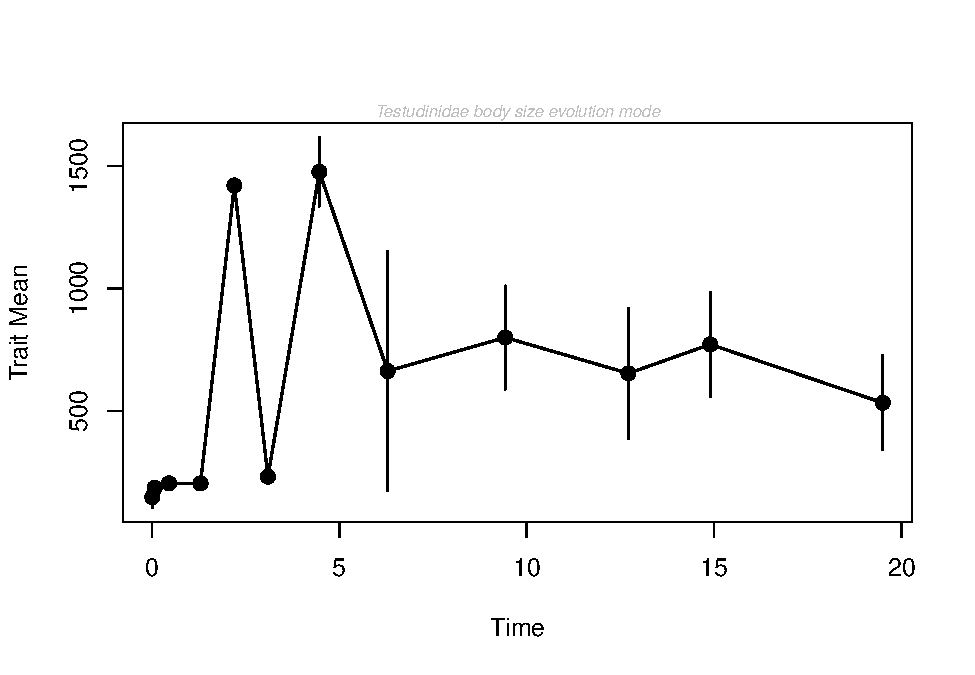
\includegraphics{MA_JJ_files/figure-latex/pTSEuC-1.pdf}
	\caption[PaleoTS plot of continental \T in Europe]{Evolutionary trajectory of Testudinidae body size on mainland Europe. Bars respresent standard errors of mean. The dashed line depicts the mean carapace length averaged across all time bins. The triangles indicate the Pleistocene/Pliocene and Pliocene/Miocene borders, respectively. Body size seems to remain largely unchanged during the Miocene, then fluctuate strongly during the Pliocene and drop sharply in the Pleistocene.}
	\label{fig:pTSEuC}
\end{figure}

\begin{longtable}[]{@{}lrrrr@{}}
	\caption[Model fits for continental \T in Europe]{Model-fitting results for continental testudinids in Europe. Stasis is the best supported model.}
	\label{tab:pTSEuCEM}\tabularnewline
	\toprule
	& logL & K & AICc & Akaike.wt\tabularnewline
	\midrule
	\endfirsthead
	\toprule
	& logL & K & AICc & Akaike.wt\tabularnewline
	\midrule
	\endhead
	GRW & -87.93137 & 2 & 181.3627 & 0.009\tabularnewline
	URW & -92.56882 & 1 & 187.5821 & 0.000\tabularnewline
	Stasis & -83.21073 & 2 & 171.9215 & 0.991\tabularnewline
	\bottomrule
\end{longtable}


\FloatBarrier

%__________________________________________________________________________


\subsubsection*{Europe, genera,
	insular}\label{europe-genera-insular}

\begin{longtable}[]{@{}rrrr@{}}
	\caption[PaleoTS object of insular \T in Europe]{PaleoTS object of insular testudinids in Europe. Mean Age (tt), sample size (nn), mean carapace lengths (mm) and variance (vv) are shown. Largest mean carapace length occurs in the Upper Miocene.}
	\label{tab:pTSEuI}\tabularnewline
	\toprule
	tt & nn & mm & vv\tabularnewline
	\midrule
	\endfirsthead
	\toprule
	tt & nn & mm & vv\tabularnewline
	\midrule
	\endhead
	0.00585 & 1 & 187.5077 & 0.00\tabularnewline
	0.06885 & 2 & 831.5000 & 684.50\tabularnewline
	0.45350 & 1 & 722.5000 & 0.00\tabularnewline
	1.29350 & 4 & 835.0833 & 168423.36\tabularnewline
	2.19700 & 2 & 1005.0000 & 1462050.00\tabularnewline
	3.09400 & 3 & 451.6667 & 40558.33\tabularnewline
	4.46600 & 2 & 826.1667 & 15196.06\tabularnewline
	6.28900 & 1 & 1850.0000 & 0.00\tabularnewline
	\bottomrule
\end{longtable}

\begin{figure}[H]
	\centering
	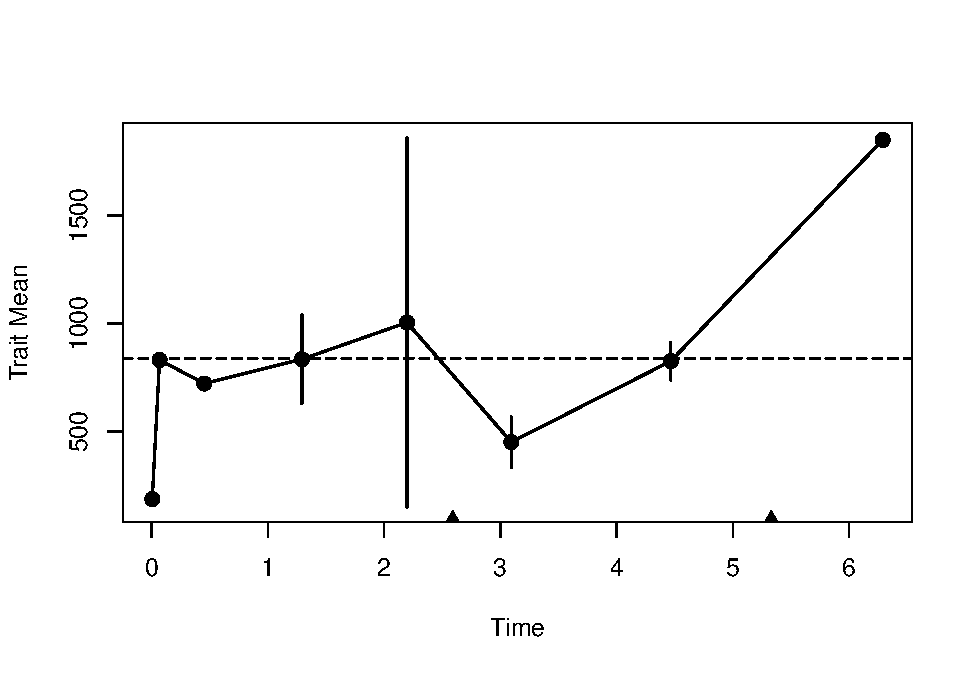
\includegraphics{MA_JJ_files/figure-latex/pTSEuI-1.pdf}
	\caption[PaleoTS plot of insular \T in Europe]{Evolutionary trajectory of Testudinidae body size on European islands. Bars respresent standard errors of mean. The dashed line depicts the mean carapace length averaged across all time bins. The triangles indicate the Pleistocene/Pliocene and Pliocene/Miocene borders, respectively. Body size decreases starting from the Upper Miocene, increases slightly during the Pleistocene and then drops sharply during the Holocene.
	}
	\label{fig:pTSEuI}
\end{figure}

\begin{longtable}[]{@{}lrrrr@{}}
	\caption[Model fits for insular \T in Europe]{Model-fitting results for insular testudinids in Europe. Stasis is the best supported model.}
	\label{tab:pTSEuIEM}\tabularnewline
	\toprule
	& logL & K & AICc & Akaike.wt\tabularnewline
	\midrule
	\endfirsthead
	\toprule
	& logL & K & AICc & Akaike.wt\tabularnewline
	\midrule
	\endhead
	GRW & -67.12192 & 2 & 141.2438 & 0.000\tabularnewline
	URW & -57.51634 & 1 & 117.8327 & 0.074\tabularnewline
	Stasis & -52.89638 & 2 & 112.7928 & 0.926\tabularnewline
	\bottomrule
\end{longtable}

\FloatBarrier
%_________________________________________________________________________




\subsubsection*{Eurasia, genera,
	continental}\label{eurasiagenera-continental}

\begin{longtable}[]{@{}rrrr@{}}
	\caption[PaleoTS object of continental \T in Eurasia]{PaleoTS object of continental testudinids in Eurasia. Mean Age (tt), sample size (nn), mean carapace lengths (mm) and variance (vv) are shown. Largest mean carapace length occurs in the Upper Miocene and throughout the Pliocene.}
	\tabularnewline
	\toprule
	tt & nn & mm & vv\tabularnewline
	\midrule
	\endfirsthead
	\toprule
	tt & nn & mm & vv\tabularnewline
	\midrule
	\endhead
	0.00585 & 6 & 210.6223 & 10502.932\tabularnewline
	0.06885 & 2 & 228.5000 & 3444.500\tabularnewline
	0.45350 & 2 & 205.4750 & 198.005\tabularnewline
	1.29350 & 4 & 595.5388 & 191487.404\tabularnewline
	2.19700 & 4 & 1044.5833 & 442006.250\tabularnewline
	3.09400 & 3 & 1110.8333 & 581102.083\tabularnewline
	4.46600 & 4 & 1159.0000 & 439728.667\tabularnewline
	6.28900 & 3 & 1092.2500 & 788605.188\tabularnewline
	9.42700 & 6 & 800.0508 & 263434.389\tabularnewline
	12.71400 & 5 & 653.9625 & 351634.528\tabularnewline
	14.89500 & 5 & 772.0000 & 223154.375\tabularnewline
	19.50000 & 5 & 513.8533 & 162399.349\tabularnewline
	\bottomrule
\end{longtable}

\begin{figure}[H]
	\centering
	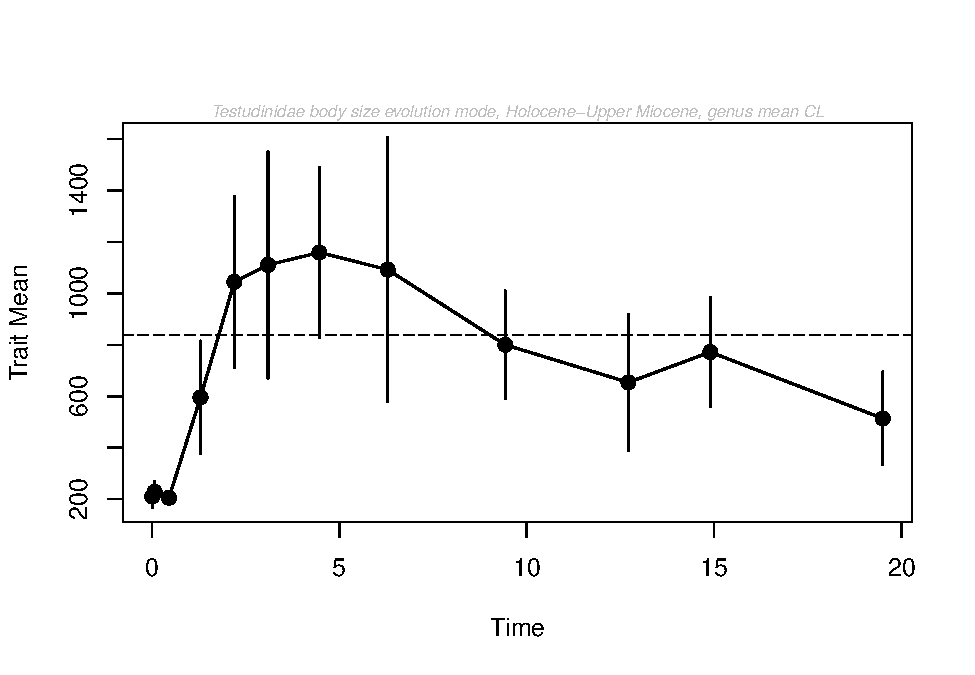
\includegraphics{MA_JJ_files/figure-latex/pTSEsC-1.pdf}
	\caption[PaleoTS plot of continental \T in Eurasia]{Evolutionary trajectory of Testudinidae body size on mainland Eurasia. Bars respresent standard errors of mean. The dashed line depicts the mean carapace length averaged across all time bins. The triangles indicate the Pleistocene/Pliocene and Pliocene/Miocene borders, respectively. Body size seems to constantly increase during the Miocene, peak during the Pliocene and then steadilydecline during the Pleistocene.}
	\label{fig:pTSEsC}
\end{figure}

\begin{longtable}[]{@{}lrrrr@{}}
	\caption[Model fits for continental \T in Eurasia]{Model-fitting results for continental testudinids in Eurasia. URW is the best supported model.}
	\label{tab:pTSEsC}
	\tabularnewline
	\toprule
	& logL & K & AICc & Akaike.wt\tabularnewline
	\midrule
	\endfirsthead
	\toprule
	& logL & K & AICc & Akaike.wt\tabularnewline
	\midrule
	\endhead
	GRW & -74.89025 & 2 & 155.2805 & 0.211\tabularnewline
	URW & -75.10165 & 1 & 152.6477 & 0.787\tabularnewline
	Stasis & -79.85118 & 2 & 165.2024 & 0.001\tabularnewline
	\bottomrule
\end{longtable}


\FloatBarrier
%__________________________________________________________________________

\subsubsection*{Eurasia, genera,
	insular}\label{eurasiagenera-insular}

\begin{longtable}[]{@{}rrrr@{}}
	\caption[PaleoTS object of insular \T in Eurasia]{PaleoTS object of insular testudinids in Eurasia. Mean Age (tt), sample size (nn), mean carapace lengths (mm) and variance (vv) are shown. Largest mean carapace length occurs in the Upper Miocene.}
	\tabularnewline
	\toprule
	tt & nn & mm & vv\tabularnewline
	\midrule
	\endfirsthead
	\toprule
	tt & nn & mm & vv\tabularnewline
	\midrule
	\endhead
	0.00585 & 4 & 272.9348 & 14139.94\tabularnewline
	0.06885 & 2 & 831.5000 & 684.50\tabularnewline
	0.45350 & 1 & 722.5000 & 0.00\tabularnewline
	1.29350 & 5 & 876.4427 & 134870.49\tabularnewline
	2.19700 & 3 & 1178.3333 & 821158.33\tabularnewline
	3.09400 & 3 & 451.6667 & 40558.33\tabularnewline
	4.46600 & 2 & 826.1667 & 15196.06\tabularnewline
	6.28900 & 1 & 1850.0000 & 0.00\tabularnewline
	\bottomrule
\end{longtable}

\begin{figure}[H]
	\centering
	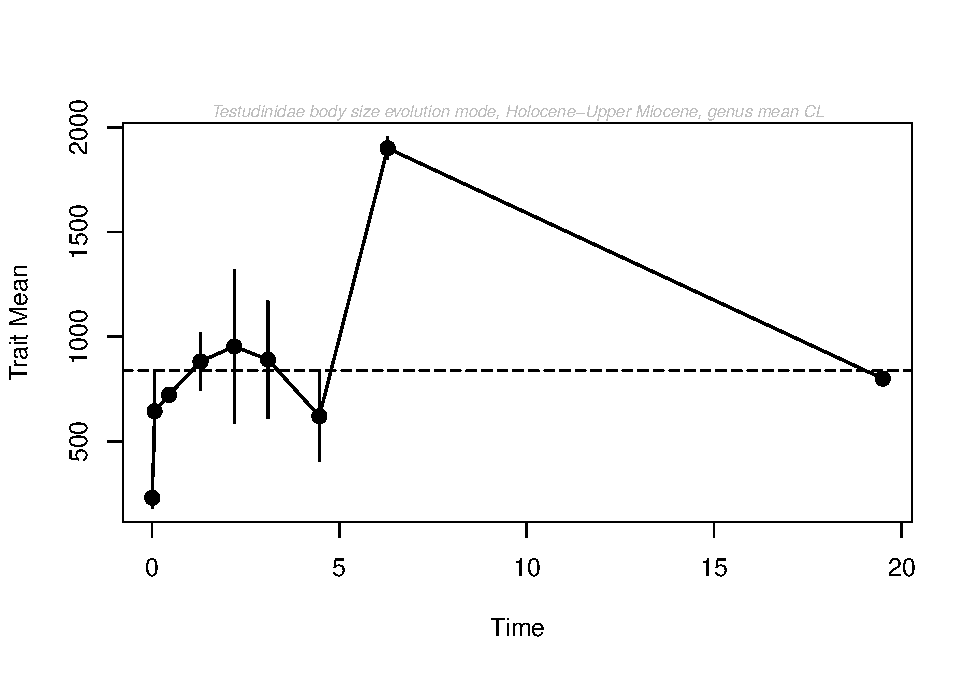
\includegraphics{MA_JJ_files/figure-latex/pTSEsI-1.pdf}
	\caption[PaleoTS plot of insular \T in Eurasia]{Evolutionary trajectory of Testudinidae body size on Eurasian islands. Bars respresent standard errors of mean. The dashed line depicts the mean carapace length averaged across all time bins. The triangles indicate the Pleistocene/Pliocene and Pliocene/Miocene borders, respectively. Body size decreases starting from the Upper Miocene, peaks shortly during the Lower Pleistocene and then drops sharply during the Holocene.
	}
	\label{fig:pTSEsI}
\end{figure}

\begin{longtable}[]{@{}lrrrr@{}}
	\caption[Model fits for insular \T in Eurasia]{Model-fitting results for insular testudinids in Eurasia. Stasis is the best supported model.}
	\label{tab:pTSEsI}
	\tabularnewline
	\toprule
	& logL & K & AICc & Akaike.wt\tabularnewline
	\midrule
	\endfirsthead
	\toprule
	& logL & K & AICc & Akaike.wt\tabularnewline
	\midrule
	\endhead
	GRW & -56.16352 & 2 & 119.3270 & 0.027\tabularnewline
	URW & -63.16971 & 1 & 129.1394 & 0.000\tabularnewline
	Stasis & -52.56060 & 2 & 112.1212 & 0.973\tabularnewline
	\bottomrule
\end{longtable}


\FloatBarrier






